W tym rozdziale omówione zostały podstawy teoretyczne dotyczące infrastruktury geodezyjnej niezbędnej do określania
połorzenia punktów a zatem i obiektów w przestrzeni. Na początku zostały omówione zagadnienia dotyczące geodezji kosmicznej,
której techniki zrewolucjonizowały możliwości człowieka w dziedzinie nawigacji tak bardzo istotnej dla rolnictwa precyzyjnego.
W pracy zdecydowano się opisać tylko trzy najpopularniejsze systemy globalnego pozycjonowania.
W dalszej części rozdziału opisano pokrótce algorytmy wyznaczania pozycji w nawigacji satelitarnej oraz inercjalnej, a tekże metodę 
integracji tych dwóch jakże uzupełniających się technik. 

\section{Układ Odniesienia}
Przykładem obrazującym potrzebę posiadania stabilnego w czasie i przestrzeni układu odniesienia są ścieżki przejazdowe,
dzięki którym koła pojazdu nie niszczą upraw. Aby możliwe było tworzenie ścieżek przejazdowych dokładność pozycjonowania 
traktora bądź innego narzędzia musi być rzędu kilku centymetrów względem poprzednich przejazdów. Jedynym sposobem 
na uzyskanie wyżej wymienionej dokładności prowadzenia maszyn jest dysponowanie precyzyjnie zdefiniowanym 
układem, w którym przechowywane będą współrzędne poprzednich przejazdów i w którym będzie dostarczana pozycja w 
czasie rzeczywistym. Ponieważ dokładność wyznaczenia pozycji w danym układzie zależy od dokładności realizacji tego układu,
w praktyce przyjmuje się, że układ odniesienia powinien być zrealizowany o rząd wielkości dokładniej niż wymagana dokładność pozycjonowania. \cite[][strona 210]{ggos}
Poniżej opisano dwa najważniejsze systemy odniesień przestrzennych oraz ich realizacje.
	\subsection{ICRS}
International Celestial Reference System - Międzynarodowy Niebieski System Odniesienia realizowany poprzez technikę VLBI - interferometria długich baz, 
składa się z zestawu procedur i konwencji oraz odpowiednich zasad modelowania koniecznych do zdefiniowania w dowolnym momencie czasu trzech osi kartezjańskiego 
układu współrzędnych w przestrzeni kosmicznej \cite{IERS_ICRS}. Osie tego układu są zdefiniowane w taki sposób aby ich kierunki wzgledem najodleglejszych obiektów 
kosmosu były stałe. Z punktu widzenia kinematyki system jest quasi-inercjalny \cite[][strona 23]{KRYNSKI_SYSTEMY}.
System jest zrealizowany fizycznie za pomocą układu odniesienia ICRF - International Celestial Reference Frame, który składa się z zbioru precyzyjnie
wyznaczonych współrzędnych pozagalaktycznych obiektów takich jak: kwazary oraz aktywne jądra niektórych galaktyk.
Ruchy własne powyższych radioźródeł są zaniedbywalne z punktu widzenia docelowej dokładności wyznaczania współrzędnych.\cite[][strona 21]{IERS_2010}.
Początek układu współrzędnych w systemie ICRS został zdefiniowany w punkcie barycentrum układu słonecznego. \cite[][strona 163]{BRZEZINSKI_2012}.
Profesorowie Brzeziński oraz Rogowski powiadają, że dokładność kierunku osi układu ICRF waha się w granicach 20 mikrosekund miary łukowej
(50 odpowiada 1.5 mm na pow. Ziemi), co przy dostępności 
precyzyjnego modelu precesji - nutacji pozwala stwierdzić, że ICRF jest najlepszym inercjalnym układem odniesienia dostępnym obecnie\cite[][strona 164]{BRZEZINSKI_2012}.
Warto zadać pytanie: dlaczego system ICRS wraz z jego realizacją w postaci ICRF są takie ważne z punktu widzenia rolnictwa precyzyjnego?
Według autorów pracy \cite[][strona 164]{BRZEZINSKI_2012} ponieważ z wystarczającą dokładnością możemy przyjać iż, układ ICRF jest inercjalny, 
są w nim zatem spełnione równania \ref{satellite_eq} ruchu sztucznych satelitów Ziemi wolne od tzw. pozornych sił bezwładności.
\begin{equation} \label{satellite_eq}
\quad \vec{ \ddot{r} } + \mu \frac{ \vec{r} } { \lvert { \vec{r} }^{\,3} \rvert } = \vec{a_p}
\end{equation} 
Gdzie $ \vec{r} $ oznacza pozycję satelity względem środka mas Ziemi.\\
$\vec{ddot{r}}$ oznacza drugą pochodną wektora względem czasu.\\
$\mu = GM $ oznacza ziemską stałą grawitacji.\\
$\vec{a_p}$ wyraża przyspieszenia perturbujące np. pochodzące od promieni słonecznych.
Według autorów opracowania \cite[]{BRZEZINSKI_2012} po uprzednim scałkowaniu równania różniczkowego \ref{satellite_eq}
otrzymujemy chwilową pozycję satelity w inercjalnym systemie ICRS. Jedną z fundamentalnych funkcji systemu ICRS 
jest zatem dostarczanie odniesienia podczas wyznaczeń orbit sztucznych satelitów Ziemi. Punkty aproksymujące dyskretnie orbitę satelity 
są transformowane do systemu ITRS (patrz następny paragraf) w którym to systemie są publikowane gotowe produkty IGS. ( orbity + parametry zegarów).
Powyższą transformację opisano np. w monografi \cite[][strona 43]{IERS_2010}. Transformacja jest realizowana w oparciu o ruchy bieguna niebieskiego,
model precesji oraz nutacji a także ruchy bieguna ziemskiego. Warto zwrócić uwagę na fakt znacznego pogorszenia dokładności opisanej transformacji,
gdy jest ona wykonywana w czasie rzeczywistym w zastosowaniach nawigacyjnych. Dla przykładu wpływ pływów skorupy ziemskiej daje efekt rzędu 
$\frac{+}{-}25 cm$ \cite[][strona 166]{BRZEZINSKI_2012}. W różnicowych algorytmach pozycjonowania (RTK, DGPS etc.) 
efekty takie nie mają wielkiego znaczenia, natomiast w pomiarach absolutnych (ppp) wymagane jest ich jak najlepsze modelowanie.
	%%%%%%%%%%%%%%%%%%%%%
	\subsection{ITRS}
	%%%%%%%%%%%%%%%%%%%%%%
Terrestial Reference System - Ziemski System Odniesienia jest to system odniesień przestrzennych wirujący wraz z Ziemią w jej dziennym ruchu w 
przestrzeni kosmicznej. W systemie tym pozycje punktów są ścieśle związane z powierzchnią Ziemi i podlegają niewielkim wariacjom powodowanym przez efekty geofizyczne, 
takie jak ruchy płyt tektonicznych i pływy skorupy ziemskiej oraz pływy oceaniczne \cite[][strona 34]{IERS_2010}.
W wielkim skrócie można powiedzieć, że Ziemski System Odniesienia składa się z konwencji regulujących początek, skalę oraz orientację układu odniesienia.
International Terrestial Reference system - Międzynarodowy Ziemski System Odniesienia definiuje powyższe parametry w następujacy sposób:
\begin{itemize}
\item Początek układu współrzędnych powinien znajdować się w punkcie tzw. geocentrum - środek mas Ziemi wraz z oceanami oraz atmosferą \cite[]{IERS_2010}.
\item TCG - Czas współrzędnych geocentrycznych jako system czasu. Skala układu odniesienia ma być zgodna z definicją czasu TCG. Za jednostkę 
długości przyjęto metr (SI) \cite[]{IERS_2010}.
\item Orientacja przestrzenna zgodna z wyznaczeniami BIH na epokę 1984. \cite[]{IERS_2010}.
\item Zmienność w czasie orientacji przestrzennej określana na podstawie warunku, iż globalna suma poziomych ruchów tektonicznych nie zawiera składowych 
obrotu \cite[]{IGIK_ITRS}.
\end{itemize}
Fizyczną realizacją systemu ITRS jest Międzynarodowy Ziemski Układ Odniesienia (ITRF). Układ ten powstał z integracji obserwacji wykonanych technikami VLBI, 
SLR, LLR, DORIS oraz szeregów czasowych wyznaczeń pozycji stacji referencyjnych GPS. 
Aktualną wersją systemu jest ITRF2008, przedstawiony na rysunku \ref{fig:ch2_itrf_2008}. 
\begin{figure}[H]
\centering
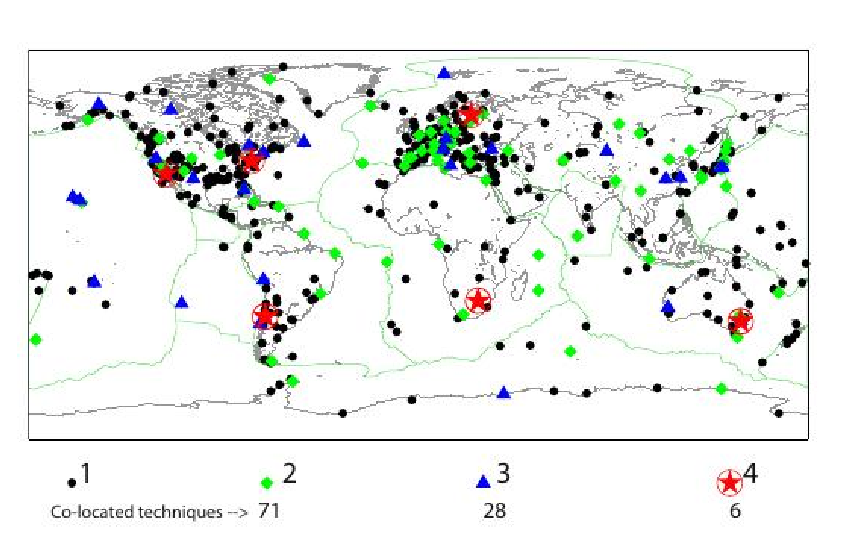
\includegraphics[scale=0.7]{ch2_ITRF_2008.eps}
\caption{\textit{Sieć stacji referencyjnych tworząca układ ITRF2008} źródło: \cite[][strona 38]{IERS_2010}}
\label{fig:ch2_itrf_2008}
\end{figure}
Układ ITRF składa się z współrzędnych oraz prędkości wybranych stacji referencyjnych oraz ich macierzy kowariancji. Parametry te są wyznaczane 
w centrach obliczeniowych Międzynarodowej Służby Ruchu Obrotowego Ziemi oraz Systemów Odniesienia (IERS) i publikowane w IERS Conventions. \cite[][strona 167]{ROCZNIK_2014}.
Warto jeszcze raz podkreślić, że dokładność wszystkich produktów służby IGS (International GNSS Service) takich jak orbity satelitów jest determinowana 
przez dokładność układu odniesienia do jakiego są one transformowane ( z układu niebieskiego ICRF) i następnie publikowane. Dokładność produktów IGS 
ma bezpośredni wpływ na wynik rozwiązania pozycji podczas nawigacji w czasie rzeczywistym.
Układ odniesienia IGS jest determinowany na podstawie tylko obserwacji GNSS wykonywanych na starannie wyselekcjonowanym podzbiorze 
stacjach referencyjnych IERS, i wpasowywany następnie za pomocą 14 parametrowej transformacji Helmerta do układu ITRF2008 \cite[]{ALTAMIMI_2009}.
Globalny układ odniesienia IGS jest zatem zgodny z układem ITRF2008. Ponadto wszystkie dane powstałe przed rokiem 2008 zostały odpowiednio 
przetransformowane w celu osiągnięcia jak największej wewnętrznej spójności \cite[][strona 15]{KOUBA_2009}.
Dla lepszego zrozumienia dalszych rozdziałów kluczowe wydaje się wyjaśnienie, że współrzędne stacji referencyjnych w układzie ITRF 
są wolne od wpływu pływów oceanicznych, pływów skorupy ziemskiej, oraz zmian położenia osi obrotu Ziemi (tzw. ruch bieguna).
W sensie globalnym pozycja każdej stacji referencyjnej podlega periodycznym fluktuacjom których amplituda jest rzędu kilku
decymetrów. W układzie ITRF powyższe wysokie częstotliwości są eliminowane za pomocą zastosowanych modeli. W pomiarach względnych o krótkich
bazach (<100km) fluktuacje są w przybliżeniu takie same, zatem do współrzędnych ITRF nie jest konieczne wprowadzanie poprawek.
Poprawki są jednak konieczne gdy wykonujemy pomiary w sensie absolutnym (aktualną pozycję wyznaczamy bezpośrednio względem znanych orbit)
w technice PPP lub w przypadku gdy pomiary różnicowe wykonywane są dla dużych odległości. \cite[][strona 11]{KOUBA_2009}

\section{Globalne Systemy Nawigacji Satelitarnej GNSS}
\noindent Znaczenie akronimu GNSS (Global Navigation Satellite Systems) nie jest jednoznaczne. Większość środowiska naukowego 
postrzega ostatni wyraz skrótu w liczbie mnogiej - systemy, takiej też interpretacji przyjęto używać w niniejszej pracy.
Dzieje się tak ponieważ, jest kilka systemów satelitarnego pozycjonowania. Większość z nich 
została opisana pokrótce w dalszej częsći tego podrozdziału. Jednakże jeżeli spojrzymy na systemy GNSS z punktu widzenia rozwiązania 
nawigacyjnego bazującego na sygnałach pochodzących od różnych satelitów ( w sensie przynależności do konkretnego systemu), wtedy jako całość 
tworzą one jeden globalny system nawigacji satelitarnej \cite[][strona vii]{hofmann_gnss}.\\
\indent Systemy GNSS są sukcesorami systemów dopplerowskich - systemu Transit\footnote{Pierwszy
działający system nawigacji satelitarnej, używany przez marunarkę wojenną USA 
do określania pozycji okrętów podwodnych z dokładnością 25m. Działanie oparte na efekcie Dopplera.} oraz Cikada\footnote{Stworzony przez naukowców byłego ZSRR 
jako odpowiednik systemu Transit}, Bazują na od około 30 do 45 satelitów umieszczonych na tzw. średnich orbitach MEO\footnote{MEO 
(Medium Earth Orbit) - średnia orbita okołoziemska w której wysokość satelity względem Ziemi waha się od 2000km do 35786km - wysokość orbity geostacjonarnego)}
oraz emitujących fale radiowe w zakresie mikrofalowym na dwóch lub więcej częstotliwościach.
Pasmo mikrofalowe pozwala na używanie systemów niezależnie od panujących warunków pogodowych, natomiast sygnał emitowany na przynajmniej dwóch częstotliwosciach 
pozwala na eliminację negatywnego wpływu refrakcji jonosferycznej \cite[][strona 33]{ggos}. Quasi-symultaniczna obserwacja przez odbiornik kilku różnych 
satelitów GNSS eliminuje w znacznym stopniu błąd zegara odbiornika. Wszystkie systemy GNSS są pasywne - odbiornik nie musi wysyłać żadnych sygnałów do satelitów w 
celu wykonania pomiaru. Opisane właściwości uczyniły systemy GNSS niejako \enquote{koniami pociągowymi} nawigacji oraz geodezji kosmicznej \cite[][strona 36]{ggos}.\\
\indent W każdym systemie GNSS wyróżnić można trzy główne części: segment kosmiczny, segment użytkowników oraz segment kontrolny.
Zadaniem segmentu kosmicznego jest zapewnienie takiej konstelacji satelitów, która pozwoli na określanie pozycji oraz prędkości
użytkownika niezależnie od jego połorzenia na Ziemi.
Segment kontrolny steruje całym systemem poprzez uaktualnianie danych komputerów pokładowych satelitów oraz ochroną systemu przed nieautoryzowanymi użytkownikami.\\
\indent Należy dodać, że istanieje cały szereg systemów wspomagania GNSS w zastosowaniach nawigacyjnych, które podobnie dzielimy na kosmiczne - SBAS\footnote{
SBAS - space based augmentation systems} oraz naziemne - GBAS\footnote{GBAS - ground based augmentation systems}.
Kosmiczne systemy wspomagania składają się z sieci naziemnych stacji referencyjnych generujących poprawki różnicowe oraz informacje o sprawności systemu GNSS, 
które są dystrybuowane za momocą satelitów geostacjonarnych. W systemach GBAS odbiorniki referencyjne montowane są jedynie w pobliżu lotnisk, a poprawki 
transmitowane są drogą radiową. Przykładami SBAS są Europejski system EGNOS\footnote{EGNOS - European Geostationary Navigation Overlay Service.} 
oraz system WAAS\footnote{Wide Area Augmentation System} obejmujący swoim zasięgiem Amerykę Północną. 
	\subsection{GPS}
\noindent System GPS został stworzony przez Departament Obrony USA z myślą o wyznaczaniu pozycji, prędkości oraz synchronizacji czasu obiektów wojskowych
w globalnym układzie odniesienia, niezależnie od warunków pogodowych oraz lokalizacji użytkownika na Ziemi \cite[][strona 309]{hofmann_gnss}.
System GPS zarządzany przez Siły Powietrzne USA, osiągnął pełną operacyjność 17 lipca 1995r. System składa się z segmantu kosmicznego, kontrolnego oraz z segmantu użytkowników.
Segmant kosmiczny tworzy konstelacja satelitów GPS transmitujących sygnały radiowe do użytkowników. Rząd Stanów Zjednoczonych zobowiązał się do 
utrzymywania w przestrzeni kosmicznej minimum 24 satelity w ciągu 95\% czasu. Obecnie w przestrzeni znajduje się 31 satelitów krążących wokół Ziemi na 
wysokości około 20200km, z których wyróżniamy 27 satelitów bazowych czynnych w załorzeniu nieprzerwanie. 
Każdy obiega naszą planetę dwókrotnie w ciągu doby, poruszając się na jednej z sześciu orbit kołowych rozmieszczonych równomiernie co 60\degree,
nachylonych względem płaszczyzny równika pod kątem 55\degree \cite[]{GPS_GOV}. Poniżej na rysunku \ref{fig:gps_space_segment} przedstawiono operacyjne satelity systemu GPS
bloku II.
\begin{figure}[H]
\centering
\begin{subfigure}{.2\textwidth}
  \centering
  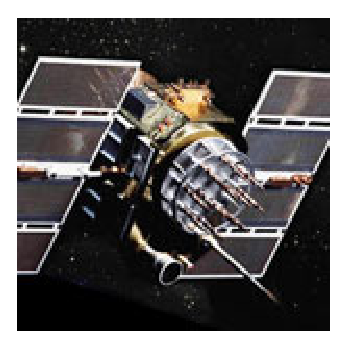
\includegraphics[width=.9\linewidth]{chapter2_gps_space_1.eps}
  \caption{blok IIa}
  \label{fig:block2a}
\end{subfigure}%
\begin{subfigure}{.2\textwidth}
  \centering
  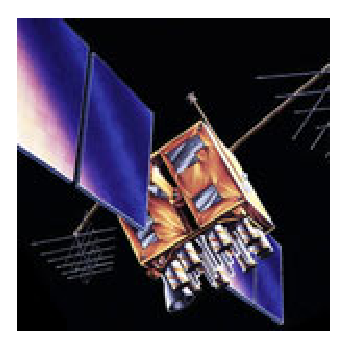
\includegraphics[width=.9\linewidth]{chapter2_gps_space_2.eps}
  \caption{blok IIR}
  \label{fig:block2r}
\end{subfigure}
\begin{subfigure}{.2\textwidth}
        \centering
        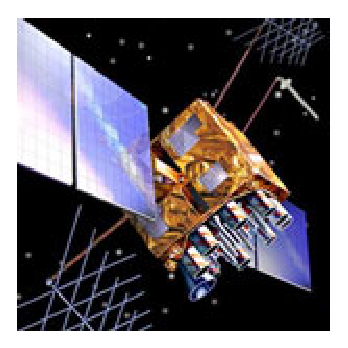
\includegraphics[width=.9\linewidth]{chapter2_gps_space_3.eps}
        \caption{blok IIR(M)}
        \label{fig:block2rm}
\end{subfigure}
\begin{subfigure}{.2\textwidth}
        \centering
        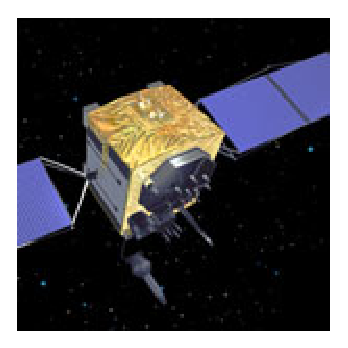
\includegraphics[width=.9\linewidth]{chapter2_gps_space_4.eps}
        \caption{blok IIF}
        \label{fig:block2f}
\end{subfigure}
\caption{\textit{Operacyjne satelity systemu GPS}
źródło: \cite[]{GPS_GOV}}
\label{fig:gps_space_segment}
\end{figure}
\indent Segment kontrolny systemu GPS składa się z sieci stacji przedstawionych na rysunku \ref{fig:gps_control_segment} ze stacją główną zlokalizowaną w stanie Colorado.
Zadaniem stacji kontrolnych jest śledzenie satelitów systemu GPS, kontrolowanie jakości transmisji danych, uaktualnianie danych oraz komputerów pokładowych znajdujących się
na satelitach oraz sterowanie konstelacją GPS. Ze względu na załorzenia niniejszej pracy segment użytkowników został zawężony głównie do rolnictwa precyzyjnego i traktuje o
nim niejako cała praca.
\begin{figure}[H]
\centering
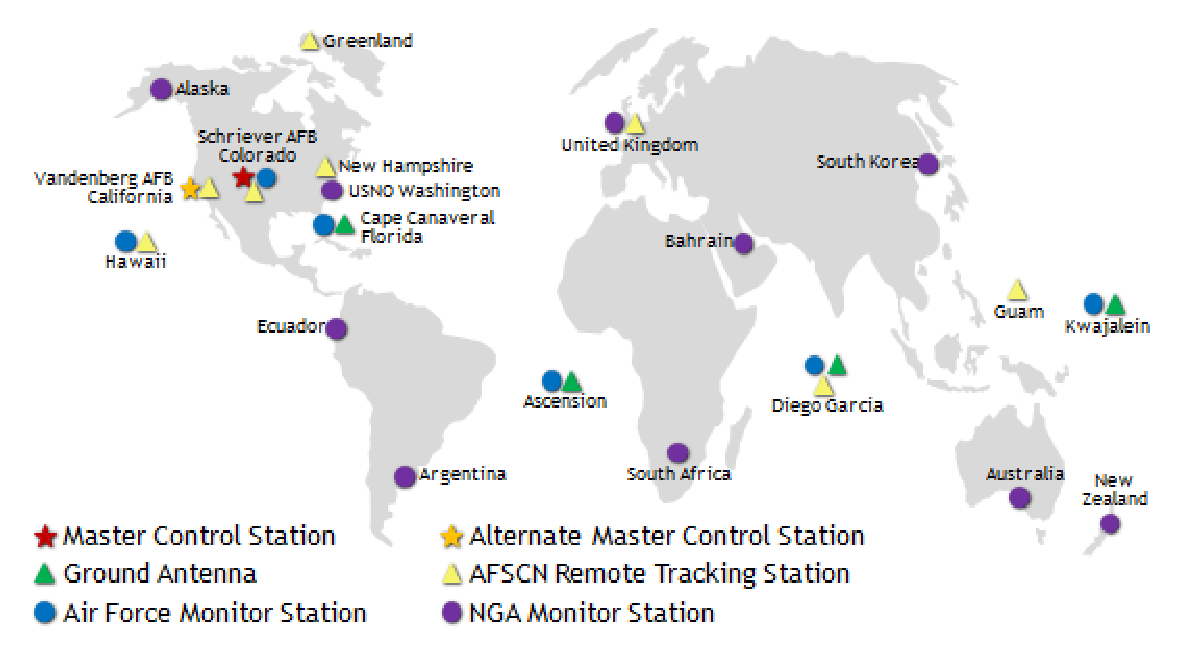
\includegraphics[scale=0.5]{chapter2_control_segment.eps}
\caption{\textit{Stacje segmentu kontrolnego GPS} źródło: \cite[]{GPS_GOV}}
\label{fig:gps_control_segment}
\end{figure}
\indent Sygnały wysyłane przez satelity dzielą się na militarne oraz do zastosowań cywilnych. Sygnały militarne są kodowane zatem w niniejszej pracy pokrótce opisano
tylko sygnały ogólnodostępne. Satelity GPS emitują fale elektromagnetyczne w paśmie radiowym. Wyróżniamy trzy częstotliwości nośne dla sygnałów GPS: 
L1 - częstotliwość podstawowa, L2 - Początkowo tylko do zastosowań wojskowych, od 2005 roku jest dostępna do zastosowań cywilnych, L5 - od kwietnia 2014r. pojawiła się 
depesza nawigacyjna dostępna użytkownikom cywilnym. Częstotliwość L5 znajduje się w paśmie radiowym zarezerwowanym dla branży lotniczej \cite[]{GPS_GOV}.
Rysunek \ref{fig:gps_freequencies} przedstawia tabelę częstotliwości nośnych GPS.
\begin{figure}[H]
\centering
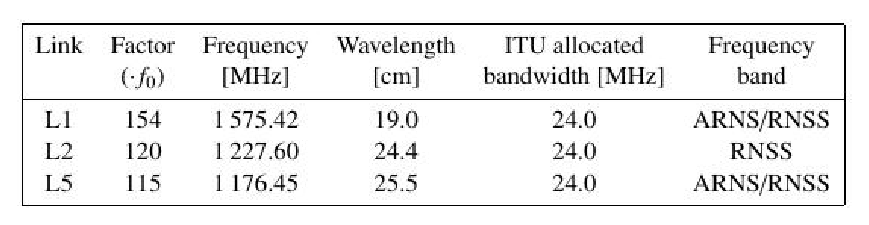
\includegraphics[scale=0.9]{chapter2_gps_freequencies.eps}
\caption{\textit{Częstotliwości nośne sygnału GPS} źródło: \cite[][strona 329]{hofmann_gnss}}
\label{fig:gps_freequencies}
\end{figure}
\noindent Bazując na powyższych częstotliwościach generowane są dane nawigacyjne w postaci tzw. kodów na których opierają się algorytmy wyznaczania pozycji odbiornika.
C/A jest kodem propagowanym na częstotliwości L1 wraz z depeszą nawigacyjną, przeznaczonym dla użytkoników cywilnych do wyznaczania pozycji w czasie rzeczywistym.
C/A jest kodem stosunkowo krótkim (297m), co pozwala na bardzo szybką inicjalizację,
lecz co za tym idzie jest bardzo łatwo podatny interferencje \cite[][strona 332]{hofmann_gnss}.
P(Y) - kod którego długość wynosi około 266.4 dni ze względu na tę właśnie cechę charakteryzuje się niemożnością jego odbierania bez apriorycznej znajomości dokładnej 
poprawki zegara, pozycji oraz efemeryd satelitów. Modulowany na dwóch częstotliwościach L1 oraz L2 kod P(Y) w zastosowaniach nawigacyjnych jest przeznaczony jedynie dla wojska.
Kodem, który jest modulowany na częstotliwości nośnej L2 i przeznaczonym do zastosowań komercyjnych jest kod L2C. Kod L2C poprzez kombinacje liniowe z kodem C/A pozwala 
na korekcję negatywnego wpływu jonosfery. Użytkownicy cywilni którzy dysponują dwuczęstotliwościowymi odbiornikami dzięki kodowi L2C są w stanie uzyskać porównywalną
dokładność jaką uzyskują użytkownicy autoryzowani na kodzie P(Y). L2C pozwala na szybszą inicjalizację odbiornika, podnosi niezawodność oraz niejako dostępność sygnału 
GPS poprzez transmisję z wyższą efektywną mocą sygnału \cite[]{GPS_GOV}. Kolejnym kodem jest L5C. Kod L5C modulowany na częstotliwośći L5 został specjalnie zaprojektowany 
aby sprostać wymaganiom aplikacji służących do celów zapewniania bezpieczeństwa życia ludzkiego \cite[][strona 335]{hofmann_gnss}. Kod L5C charakteryzuje się wysoką mocą 
sygnału oraz przepustowością danych. L5C w kombinacji z kodem C/A zwiększy istotnie dokładność poprzez eliminację wpływy jonosfery. Sygnał na częstotliwośći L5 
począwszy od 31 grudnia 2014 jest już eksperymentalnie dostępny dla użytkowników. Możliwe jest już zatem wykonywanie obserwacji sygnału GPS na trzech częstotliwościach nośnych,
co prawdopodobnie pozwoli na uzyskanie sub-metrowych dokładności bez użycia wsparcia systemów augmentacyjnych \cite[]{GPS_GOV}. W planach modernizacyjnych systemu GPS jest,
także wprowadzenie dodatkowego (oprócz C/A) kodu na częstotliwości L1 - L1C. Wprowadzenie jeszcze jednego kodu na częstotliwości L1 pozwoli na ulepszenie pozycji 
odbiorników mobilnych w miastach bądź w innych trudnych terenach. Ponadto warto zwrócić uwagę na fakt, że kod L1C został zaprojektowany wspólnie przez Europę oraz 
Stany Zjednoczone jako wspólny sygnał zarówno dla GPS jak i Galileo. Kod L1C docelowo ma być emitowany przez wszystkie dostępne systemy satelitarne \cite[]{GPS_GOV}.\\
\indent Układ odniesienia względem, którego jest wyznaczana pozycja GPS to układ WGS84\footnote{WGS84 (World Geodetic System) geocentryczny ortokartezjański układ współrzędnych
zbudowany pocztkowo w oparciu o obserwacje satelitów systemu Transit. Wraz z rozwojem technologii GPS układ został zmodernizowany czterokrotnie.
Obecna realizacja to układ WGS84(1674) z lutego 2012 roku. Obecnie układ WGS84 jest zarządzany przez jedną z agencji wywiadu USA - National Geospatial Intelligance Agency.}
,zdefiniowany poprzez wyznaczenie współrzędnych oraz prędkości stacji referencyjnych jako realizacja systemu WGS84. Współrzędne stacji referencyjnych są następnie 
używane do wyznaczanie orbit satelitów GPS. Dokładność układu WGS84 względem aktualnego układu Ziemskiego ITRF jest centymetrowa \cite[][strona 51]{donnelly}.
Należy zauważyć, że w zależności od kontekstu WGS84 odnosi się do systemu, układu odniesienia lub referencyjnej elipsoidy.
Centymetrowa dokładność aktualnej realizacji układu odniesienia systemu GPS względem układu ITRF2008 na epokę 2005
wynika bezpośrednio ze zgodności na poziomie definicyjnym systemów WGS84 oraz ITRS. Drobne różnice wynikają z tego, że do realizacji systemu WGS84 w celu uzyskania jak 
największej spójniości danych używane są jedynie obserwacje GPS. Elipsoida\footnote{Powierzchnia powstała poprzez obrót elipsy o zadanych parametrach wokół jej 
krótszej półosi. W tym konkretnym przypadku środek elipsoidy jest umieszczony w środku masy Ziemi, a jej krótsza półoś pokrywa się z osią Z układu odniesienia WGS84.}
WGS84 jest powierzchnią odniesienia aproksymującą kształt oraz rozmiary Ziemi. Różnica między elipsoidą GRS80 złączoną z układem ITRF a elipsoidą WGS84 jest z punktu 
widzenia dokładności wyznaczeń na potrzeby nawigacji, jest zaniedbywalna \cite[][strona 50]{donnelly}.\\
\indent System czasu Systemu GPS jest oparty o wzorzec czasu atomowego. Nominalnie czas GPS różni się od Międzynarodowego Czasu Atomowego TAI o 19 sekund, i jest 
ścisle związany z Uniwersalnym Czasem Koordynowanym UTC.\\
Podsumowując ten paragraf można powiedzieć, że system GPS już od ponad dwóch dekad jest nieocenionym, dla takich dziedzin działalności człowieka jak:
Budownictwo, Energetyka, Geodezja z Geodynamiką, Przemysł wydobywczy, Transport, Ratownictwo, Rolnictwo oraz wiele innych.
 	\subsection{GLONASS}
Podobnie jak system GPS powstał na podstawie doświadczeń z systemem Transit, tak system GLONASS został zbudowany z doświadczeń sowieckich naukowców 
z systemem Cikada. GLONASS jest systemem wojskowym, i podobnie jak GPS zaprojektowanym do dostarczania nielimitowanej liczbie użytkowników, niezależnie od pogody,
trójwymiarowej pozycji, synchronizacji czasu, oraz prędkości w obrębie całego globu \cite[][strona 342]{hofmann_gnss}. Operacyjność systemu ogłoszono w 1993r. 
jednakże nominalną konstelację 24 satelitów system osiągnął dopiero 18 stycznia 1996r. Z powodu kryzysu ekonomicznego Federacji Rosyjskiej liczba operacyjnych 
satelitów systematycznie spadała i w roku 2001 osiągnęła minimum w postaci liczby sprawnych satelitów poniżej dzsiesięciu \cite[][strona 342]{hofmann_gnss}.
Do pełnej operacyjności system GLONASS powrócił po około 10 latach 8 grudnia 2011 roku \cite[]{glonass_geoforum}.\\
\indent Segment kosmiczny systemu GLONASS składa się z 24 satelitów poruszających się na orbitach kołowych na wysokości około 19100km nad powierzchnią Ziemi.
Okres obiegu wokół Ziemi satelitów systemu GLONASS wynosi 11 godzin 15 minut i 44 sekundy. Konstelacja satelitów jest zgrupowana w trzech płaszczyznach o inklinacji\footnote{
Inklinacja w tym kontekście określa kąt dwuścienny między płaszczyzną orbity satelity a płaszczyzną równika.} równej 64.8\degree - w każdej znajdują się 
orbity ośmiu satelitów równomiernie rozmieszczonych (co 45\degree). Węzły wstępujące orbit satelitów należących do różnych płaszczyzn różnią się o 120\degree.
Opisana konstelacja pozwala na symultaniczną widoczność minimum pięciu satelitów z około 99\% powierzchni Ziemi \cite[][strona 349]{hofmann_gnss}.\\
\indent Segment kontrolny systemu GLONASS dzieli się na \begin{inparaenum}[1)] \item centrum sterowania systemem 
\item stacje śledzące \end{inparaenum}. Centrum sterowania systemem dzieli się na centralny moduł sychronizacyjny (Schelkowo w regionie moskiewskim) odpowiedzialny
za synchronizację czasu systemu GLONASS oraz część kontrolną (Krasnoznamensk 70km od Moskwy) gdzie ma miejsce zarządzanie wszystkimi funkcjami systemu oraz planowanie.
Stacje śledzące są podzielone na trzy grupy: \begin{inparaenum}[a)] \item cztery stacje TT\&C wspomagane pięcioma stacjami pomiarów laserowych służące do
śledzenia i monitorowania satelitów oraz wysyłania do nich wiadomości. \item cztery stacje służące do kontroli urządzeń elektronicznych. 
\item stacje optyki kwantowej \end{inparaenum}. Niestety znacząca część informacji dotyczących segmentu kontrolnego systemu GLONASS
nie jest dostępna publicznie \cite[][strona 353]{hofmann_gnss}.\\
\indent Czas systemu GLONASS jest zarządzany przez wspomniany powyżej moduł synchronizacyjny za pomocą maserów wodorowych. Czas ten jest ściśle powiązany z czasem uniwersalnym 
koordynowanym. Stałe przesunięcie wynoszące plus trzy godziny związane jest różnicą między czasem Moskiewskim oraz Greenwich. Ponadto występuje losowa 
rozbierzność nieprzekraczająca 1ms, która wynika z tego, iż wspomniane skale czasu są utrzymywane przez różne zegary \cite[][strona 346]{hofmann_gnss}.\\
\indent Jako system odniesienia systemu GLONASS oryginalnie przyjęto sowiecki SGS-85, który zamieniono w roku 1990 na SGS-90\footnote{ SGS (Soviet Geodetic System) Sowiecki 
System Odniesień Przestrzennych}. Realizacja systemu to Kartezjański układ współrzędnych otrogonalnych PE-90 zrealizowany poprzez określenie współrzędnych 26 stacji 
refrencyjnych. Różnica układu PE-90 względem układu ITRF jest dość znaczna jeżeli chodzi o wymagania dokładnościowe rolnictwa precyzyjnego.
Dla przykładu wielka półoś elipsoidy geocentrycznej PE-90 jest aż o metr krótsza od odpowiadającego parametru elipsoidy GRS80. Należy jednak zaznaczyć, że 
różnice współrzędnych punktów nie przekraczają 15 metrów (średnio 5m).
Współrzędne z układu PE-90 do układu ITRF transformuje się za pomocą transformacji siedmioparametrowej wyznaczanej za
pomocą porównania tras satelitów glonas dostępnych w obu układach odniesienia \cite[]{wgs84_pe90}.\\
\indent System GLONASS podobnie jak system GPS dostarcza wysokiej jakości sygnałów dla użytkowników autoryzowanych, oraz standardowej dokładności sygnału 
dla użytkowników cywilnych. Obecnie sygnały satelitarne systemu są przenoszone za pomocą dwóch pasm częstotliwości fali radiowej: G1 = 1602Mhz oraz G2 = 1246Mhz.
W planowanej trzeciej generacji system będzie emitował dodatkowy sygnał modulowany w paśmie częstotliwości G3 = 1204.704Mhz w podobieństwie do trzeciej częstotliwości L5 
systemu GPS. Tym co diametralnie różni system GLONASS od systemu GPS jest to, że każdy satelita moduluje swój sygnał na fali radiowej o unikalnej dla niego częstotliwości.
Na rysunku \ref{fig:glonas_freq} przedstawiona została tabela według której każdemu satelicie przyporządkowywana jest unikalna częstotliwość.
\begin{figure}[H]
\centering
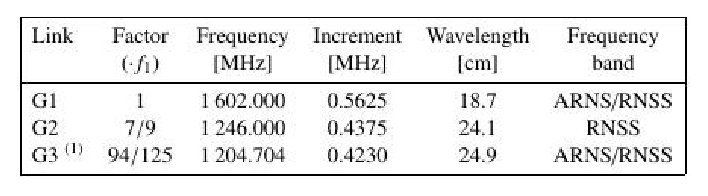
\includegraphics[scale=1.1]{chapter2_glonass_freq.eps}
\caption{\textit{Częstotliwości nośne sygnału GLONASS} źródło: \cite[][strona 357]{hofmann_gnss}}
\label{fig:glonas_freq}
\end{figure}
Tak samo jak w systemie GPS odpowiednik kodu C/A jest modulowany w paśmie częstotliwości G1 i jest nośnikiem standardowej usługi pozycjonowania.
Wysokiej dokładności sygnał P nie jset kodowany (w przeciwieństwie do GPS) i jest modulowany na obu falach nośnych G1 oraz G2. Począwszy od roku 2004 
kod standardowej dokładności jest także dostępny w paśmie G2. Na koniec warto odnotować, że pod pewnymi względami zastosowane w systemie GLONASS rozwiązania 
są lepsze niż te z systemu GPS. Większa inklinacja orbit pozwala średnio obserwować więcej satelitów, a unikalne częstotliwości sygnału dla każdego satelity 
znacząco zmniejszają niekorzystne efekty interferencji \cite[][strona 355]{hofmann_gnss}.
	\subsection{GALILEO}
System GALILEO zaprojektowano głównie na potrzeby Unii Europejskiej w celu ekonomicznego oraz strategicznego uniezależnienia jej od systemu GPS.
Ze względu na to, że system GALILEO nie jest jeszcze operacyjny (aktualnie 8 satelitów) w pracy postanowiono opisać tylko jego najważniejsze załorzenia projektowe.\\
\indent Segment kosmiczny systemu GALILEO docelowo ma się składać z 30 satelitów (27 + 3 zapasowe) po 9 satelitów operacyjnych na jedną płaszczyznę orbitalną.
Inklinacje płaszczyzn mają wynosić 56\degree. Satelity będą się poruszały po orbitach prwie kołowych na wysokości 23616km równomiernie rozmieszczone co 40\degree w 
płaszczyźnie orbity. Tak zaprojektowana konstelacja zapewnić ma globalną widoczność minimum 6 satelitów na wysokości powyżej 10\degree nad horyzontem.\\
\indent Segmant naziemny systemu GALILEO został zaprojektowany tak aby składał się z części kontrolnej stanu technicznego konstelacji satelitów oraz 
części operacyjnej, która ma odpowiadać za całościowe funkcjonowanie systemu (depesze satelitów, kontrola danych, kontrola czasu oraz wiele innych). Warto nadmienić,
że wśród stacji segmentu naziemnego oprócz klasycznej infrastruktury śledzącej satelity (kilkuczęstotliwościowe odbiorniki) znajdą się także stacje pomiarów laserowych.
\cite[][strona 380]{hofmann_gnss}. Ponadto zaprojektowano także budowę lokalnych stacji obserwacyjnych kontrolujących niezawodność systemu.\\
\indent System GALILEO ma być oparty na geocentrycznym układzie odniesienia GTRF\footnote{Galileo Terrestial Reference Frame}, który będzie powiązany z ITRF.
Z załorzeń projektowych wynika, że różnica pomiędzy GTRF oraz ITRF nie może przekraczać trzech centymetrów na poziomie ufności 2$\sigma$.\\
\indent Czas systemu GALILEO GST\footnote{Galileo System Time} będzie oparty na ciągłej skali czasu atomowego zsynchronizowanej z Międzynarodowym Czasem Atomowym TAI i
podtrzymywanej za pomocą maserów wodorowych. System czasu GALILEO będzie używał korekt czasu pochodzących od zewnętrznych ośrodków takich jak Międzynarodowe 
Biuro Miar i Wag w celu bezpośredniej synchronizacji z UTC. Maksymalna rónica midzy GST a czasem atomowym TAI ma nie przekraczać 50ns na poziomie ufności 95\%.\\
\indent Podczas projektowania systemu GALILEO przyjęto podejście nastawione na serwisy jakich system ma dostarczać użytkownikom.
Adekwatnie do potencjalnego zapotrzebowania na usługi wyróżniono następujące grupy:
\begin{itemize}
\item Serwis otwarty (OS) - dostępny dla wszystkich użytkowników bezpłatnie. Charakteryzuje się brakiem informacji na temat wiarygodności systemu.
Przeznaczony jest do uzyskiwania pozycji oraz referencji czasowej nie wymagających wysokiej dokładności. Sześć jawnych kodów jest modulowanych na fale radiowe o 
trzech częstotliwościach nośnych. Jednoczęstotliwościowe odbiorniki systemu GALILEO będą wyznaczać pozycję porównywalną z rozwiązaniem opartym o kod C/A GPS.
\item Serwis komercyjny (CS) - różniący się od serwisu otwartego gwarancją dostępności oraz dostępem do dodatkowych szyfrowanych danych zawieranych w depeszy nawigacyjnej 
propagowanej za pomocą modulacji sygnału na trzech częstotliwościach nośnych. 
\item Serwis bezpieczeństwa życia (SoL) - bazuje na tych samych sygnałach co serwis otwarty. W tym trybie w depeszy nawigacyjnej zawarta będzie informacja o wiarygodności 
systemu GALILEO. Jakiekolwiek awarie będą sygnalizowane odpowienimi ostrzeżeniami wysyłanymi do użytkownika.
\item Serwis publiczny regulowany (PRS) - przeznaczony dla służb, agencji rządowych bądź innych podmiotów zajmujących się ochroną obywateli, obronnością oraz dbaniem o
respektowanie prawa. Głównym celem serwisu jest dostarczanie silnego ciągłego oraz zakodowanego sygnału który będzie możliwy do użycia nawet w sytuacjach kryzysowych.
Sygnał w tym serwisie będzie modulowany na dwie częstotliwości nośne aby zmaksymalizować odporność na interferencje przy jednoczesnej minimalizacji ryzyka celowych
zakłóceń zewnętrznych. W serwisie tym będzie również dostępna informacja o wiarygodności systemu GALILEO.
\item Serwis ratunkowy (SAR) - Serwis polage na wykrywaniu przez satelity systemu sygnałów ratunkowych (406Mhz), a następnie na przesyłaniu tej informacji do 
centrum segmentu naziemnego, które ma za zadanie powiadomić odpowiednie służby.
\end{itemize}
\indent System GALILEO ma wykorzystywać trzy pasma częstotliwości fali radiowych L1, E5, E6 na których będzie możliwa modulacja dziesięciu różnych sygnałów.
Rysunek \ref{fig:galileo_freq} przedstawia schemat przydziału częstotliwości nośnych poszczególnym sygnałom systemu GALILEO.
Trzy sygnałý nawigacyjne modulowane na częstotliwości E1: Dwa nieszyfrowane sygnały E1B orax E1C dostępne dla wszystkich użytkowników. E1B oprócz wiadomości nawigacyjnej 
prtzenosić ma szyfrowane dane komercyjne oraz informacje o wiarygodności. Kanał danych E1B oraz kanał pilotażowy E1C mają wspierać usługi otwartą, komercyjną oraz 
usługę ratowania życia. Zaszyfrowany komponent E1A ma być dostępny tylko dla autoryzowanych użytkowników w serwisie (PRS) \cite[][strona 387]{hofmann_gnss}.
Podobnie do pasma częstotliwości E1, pasmo E6 również ma być nośnikiem trzech sygnałów: E6A, E6B, E6C dostępnych komercyjnie. 
Sygnał E6B ma być nosnikiem depeszy nawigacyjnej oraz szyfrowanych danych komercyjnych. Sygnał E6C ma być kanałem pilotażowym a E6A wspierać serwis regulowany (PRS)
\cite[][strona 389]{hofmann_gnss}.
Pasmo częstotliwości E5 jest nośnikiem czterech sygnałów. W pasmach E5a oraz E5b przenoszone są dwie pary: kanał danych plus kanał pilotażowy.
\begin{figure}[H]
\centering
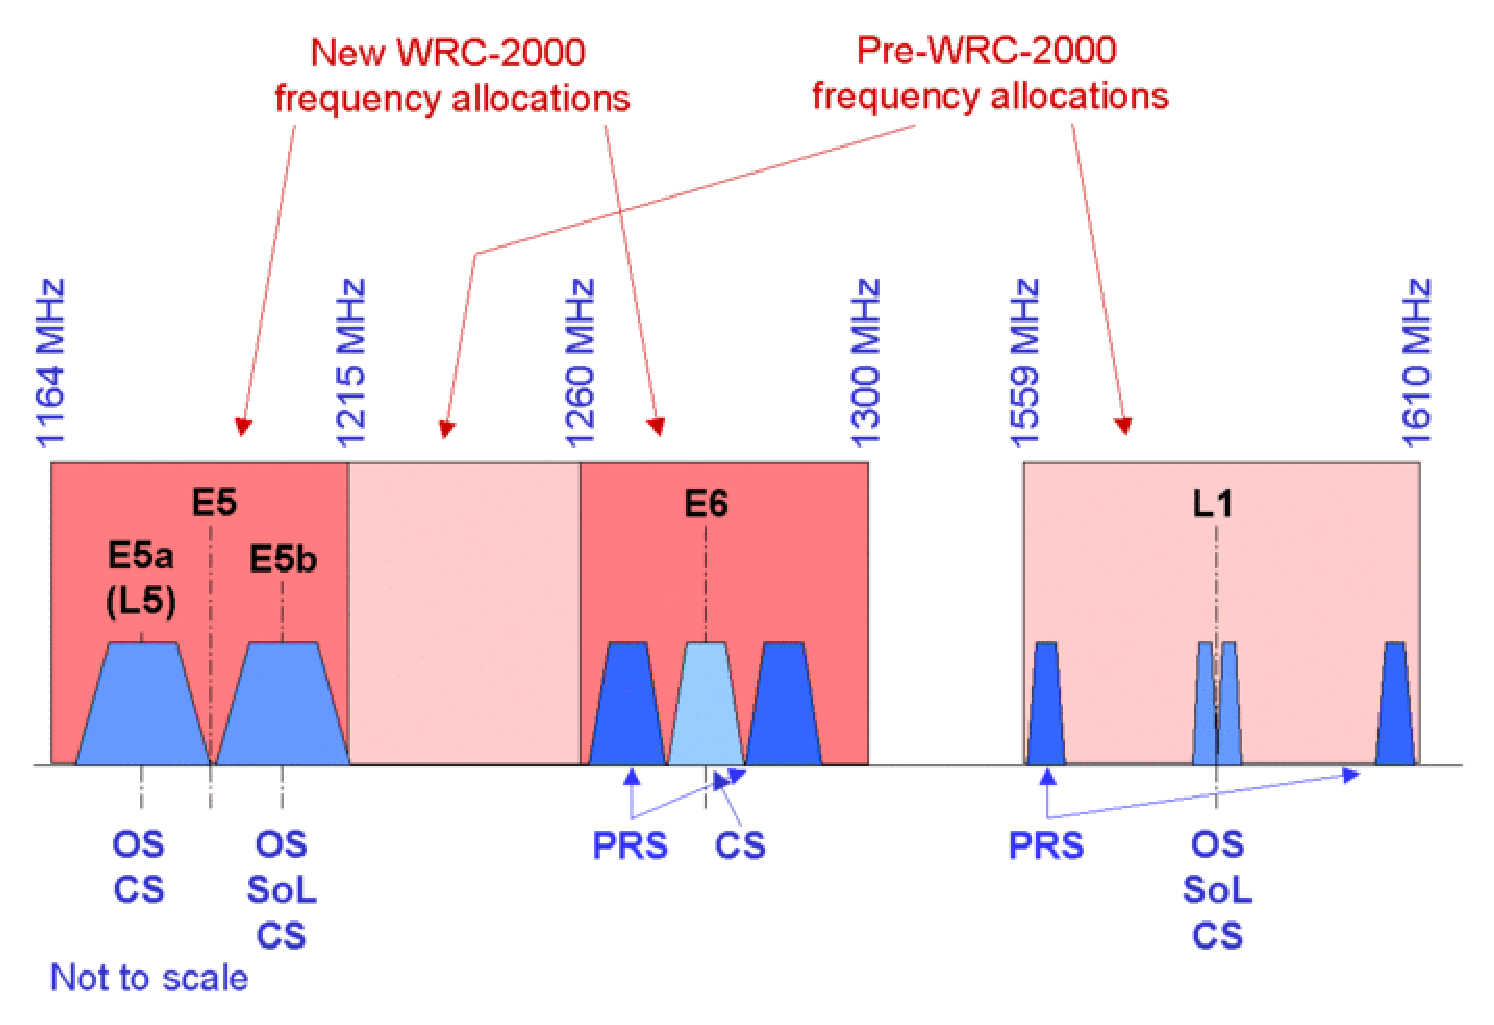
\includegraphics[scale=0.6]{chapter2_galileo_freq.eps}
\caption{\textit{Schemat częstotliwości nośnych sygnałów systemu GALILEO} źródło: \protect\url{http://www.esa.int/spaceinimages/Images/2005/04/Galileo_signal_frequencies}}
\label{fig:galileo_freq}
\end{figure}
\section{Algorytmy Pozycjonowania}

	\subsection{DGPS/DGNSS}
	\subsection{RTK}
	\subsection{PPP}
\section{Nawigacja Inercjalna}
% w tej sekcji troche o filtrze kalmana 
\noindent
Jeżeli wykorzystujemy w pomiarach pozycji DGPS – pomiar względny na podstawie pseudoodległości,
to dokładność lokalizacji pojazdu wynosi około 2m. 
Jeżeli natomiast zastosujemy technikę względnego opracowania obserwacji fazowych RTK dokładność wynosi 2cm.
Poniżej na rysunku \ref{fig:ch2_gpsReceiverExample} przedstawiono komputer z systemem wbudowanym,
który zintegrowano z odbiornikiem GPS \cite{CCTA_951_958}.
\begin{figure}[H]
\centering
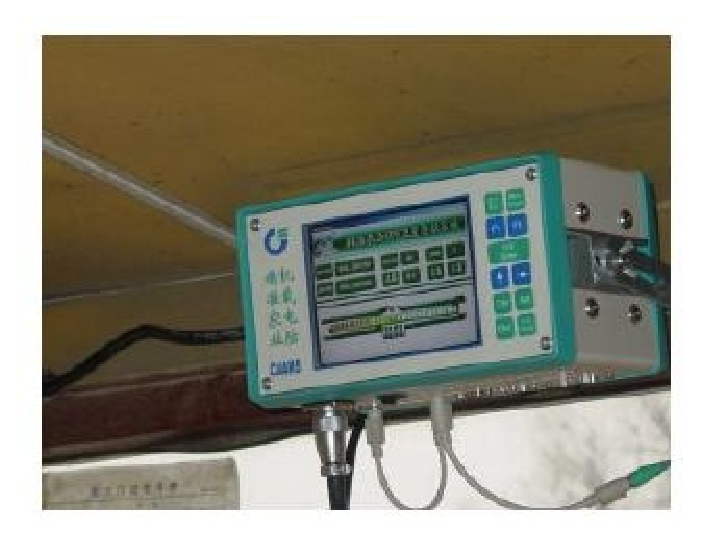
\includegraphics[scale=0.5]{ch2_gpsReceiverExample.eps}
\caption{\textit{Komputer z systemem wbudowanym, zintegrowanym z odbiornikiem GPS;} źródło: \cite[][strona 952]{CCTA_951_958}}
\label{fig:ch2_gpsReceiverExample}
\end{figure}
\noindent
%TODO trzeba opisać na czym polega filtracja Kalmana ( zaawansowane metody opracowania obserwacji)
